% !Mode:: "TeX:UTF-8"
\documentclass[12pt,a4paper]{article}

%%%%%%%%------------------------------------------------------------------------
%%%% 日常所用宏包

%% 控制页边距
% 如果是beamer文档类, 则不用geometry
\makeatletter
\@ifclassloaded{beamer}{}{\usepackage[top=2.5cm, bottom=2.5cm, left=2.5cm, right=2.5cm]{geometry}}
\makeatother

%% 控制项目列表
\usepackage{enumerate}

%% 多栏显示
\usepackage{multicol}

%% 算法环境
\usepackage{algorithm}  
\usepackage{algorithmic} 
\usepackage{float} 

%% 网址引用
\usepackage{url}

%% 控制矩阵行距
\renewcommand\arraystretch{1.4}

%% hyperref宏包,生成可定位点击的超链接,并且会生成pdf书签
\makeatletter
\@ifclassloaded{beamer}{
\usepackage{hyperref}
\usepackage{ragged2e} % 对齐
}{
\usepackage[%
    pdfstartview=FitH,%
    CJKbookmarks=true,%
    bookmarks=true,%
    bookmarksnumbered=true,%
    bookmarksopen=true,%
    colorlinks=true,%
    citecolor=blue,%
    linkcolor=blue,%
    anchorcolor=green,%
    urlcolor=blue%
]{hyperref}
}
\makeatother



\makeatletter % 如果是 beamer 不需要下面两个包
\@ifclassloaded{beamer}{
\mode<presentation>
{
} 
}{
%% 控制标题
\usepackage{titlesec}
%% 控制目录
\usepackage{titletoc}
}
\makeatother

%% 控制表格样式
\usepackage{booktabs}

%% 控制字体大小
\usepackage{type1cm}

%% 首行缩进,用\noindent取消某段缩进
\usepackage{indentfirst}

%% 支持彩色文本、底色、文本框等
\usepackage{color,xcolor}

%% AMS LaTeX宏包: http://zzg34b.w3.c361.com/package/maths.htm#amssymb
\usepackage{amsmath,amssymb}
%% 多个图形并排
\usepackage{subfig}
%%%% 基本插图方法
%% 图形宏包
\usepackage{graphicx}
\newcommand{\red}[1]{\textcolor{red}{#1}}
\newcommand{\blue}[1]{\structure{#1}}
\newcommand{\brown}[1]{\textcolor{brown}{#1}}
\newcommand{\green}[1]{\textcolor{green}{#1}}


%%%% 基本插图方法结束

%%%% pgf/tikz绘图宏包设置
\usepackage{pgf,tikz}
\usetikzlibrary{shapes,automata,snakes,backgrounds,arrows}
\usetikzlibrary{mindmap}
%% 可以直接在latex文档中使用graphviz/dot语言,
%% 也可以用dot2tex工具将dot文件转换成tex文件再include进来
%% \usepackage[shell,pgf,outputdir={docgraphs/}]{dot2texi}
%%%% pgf/tikz设置结束


\makeatletter % 如果是 beamer 不需要下面两个包
\@ifclassloaded{beamer}{

}{
%%%% fancyhdr设置页眉页脚
%% 页眉页脚宏包
\usepackage{fancyhdr}
%% 页眉页脚风格
\pagestyle{plain}
}

%% 有时会出现\headheight too small的warning
\setlength{\headheight}{15pt}

%% 清空当前页眉页脚的默认设置
%\fancyhf{}
%%%% fancyhdr设置结束


\makeatletter % 对 beamer 要重新设置
\@ifclassloaded{beamer}{

}{
%%%% 设置listings宏包用来粘贴源代码
%% 方便粘贴源代码,部分代码高亮功能
\usepackage{listings}

%% 设置listings宏包的一些全局样式
%% 参考http://hi.baidu.com/shawpinlee/blog/item/9ec431cbae28e41cbe09e6e4.html
\lstset{
showstringspaces=false,              %% 设定是否显示代码之间的空格符号
numbers=left,                        %% 在左边显示行号
numberstyle=\tiny,                   %% 设定行号字体的大小
basicstyle=\footnotesize,                    %% 设定字体大小\tiny, \small, \Large等等
keywordstyle=\color{blue!70}, commentstyle=\color{red!50!green!50!blue!50},
                                     %% 关键字高亮
frame=shadowbox,                     %% 给代码加框
rulesepcolor=\color{red!20!green!20!blue!20},
escapechar=`,                        %% 中文逃逸字符,用于中英混排
xleftmargin=2em,xrightmargin=2em, aboveskip=1em,
breaklines,                          %% 这条命令可以让LaTeX自动将长的代码行换行排版
extendedchars=false                  %% 这一条命令可以解决代码跨页时,章节标题,页眉等汉字不显示的问题
}}
\makeatother
%%%% listings宏包设置结束


%%%% 附录设置
\makeatletter % 对 beamer 要重新设置
\@ifclassloaded{beamer}{

}{
\usepackage[title,titletoc,header]{appendix}
}
\makeatother
%%%% 附录设置结束


%%%% 日常宏包设置结束
%%%%%%%%------------------------------------------------------------------------


%%%%%%%%------------------------------------------------------------------------
%%%% 英文字体设置结束
%% 这里可以加入自己的英文字体设置
%%%%%%%%------------------------------------------------------------------------

%%%%%%%%------------------------------------------------------------------------
%%%% 设置常用字体字号,与MS Word相对应

%% 一号, 1.4倍行距
\newcommand{\yihao}{\fontsize{26pt}{36pt}\selectfont}
%% 二号, 1.25倍行距
\newcommand{\erhao}{\fontsize{22pt}{28pt}\selectfont}
%% 小二, 单倍行距
\newcommand{\xiaoer}{\fontsize{18pt}{18pt}\selectfont}
%% 三号, 1.5倍行距
\newcommand{\sanhao}{\fontsize{16pt}{24pt}\selectfont}
%% 小三, 1.5倍行距
\newcommand{\xiaosan}{\fontsize{15pt}{22pt}\selectfont}
%% 四号, 1.5倍行距
\newcommand{\sihao}{\fontsize{14pt}{21pt}\selectfont}
%% 半四, 1.5倍行距
\newcommand{\bansi}{\fontsize{13pt}{19.5pt}\selectfont}
%% 小四, 1.5倍行距
\newcommand{\xiaosi}{\fontsize{12pt}{18pt}\selectfont}
%% 大五, 单倍行距
\newcommand{\dawu}{\fontsize{11pt}{11pt}\selectfont}
%% 五号, 单倍行距
\newcommand{\wuhao}{\fontsize{10.5pt}{10.5pt}\selectfont}
%%%%%%%%------------------------------------------------------------------------


%% 设定段间距
\setlength{\parskip}{0.5\baselineskip}

%% 设定行距
\linespread{1}


%% 设定正文字体大小
% \renewcommand{\normalsize}{\sihao}

%制作水印
\RequirePackage{draftcopy}
\draftcopyName{XTUMESH}{100}
\draftcopySetGrey{0.90}
\draftcopyPageTransform{40 rotate}
\draftcopyPageX{350}
\draftcopyPageY{80}

%%%% 个性设置结束
%%%%%%%%------------------------------------------------------------------------


%%%%%%%%------------------------------------------------------------------------
%%%% bibtex设置

%% 设定参考文献显示风格
% 下面是几种常见的样式
% * plain: 按字母的顺序排列,比较次序为作者、年度和标题
% * unsrt: 样式同plain,只是按照引用的先后排序
% * alpha: 用作者名首字母+年份后两位作标号,以字母顺序排序
% * abbrv: 类似plain,将月份全拼改为缩写,更显紧凑
% * apalike: 美国心理学学会期刊样式, 引用样式 [Tailper and Zang, 2006]

\makeatletter
\@ifclassloaded{beamer}{
\bibliographystyle{apalike}
}{
\bibliographystyle{unsrt}
}
\makeatother


%%%% bibtex设置结束
%%%%%%%%------------------------------------------------------------------------

%%%%%%%%------------------------------------------------------------------------
%%%% xeCJK相关宏包

\usepackage{xltxtra,fontspec,xunicode}
\usepackage[slantfont, boldfont]{xeCJK} 

\setlength{\parindent}{2em}%中文缩进两个汉字位

%% 针对中文进行断行
\XeTeXlinebreaklocale "zh"             

%% 给予TeX断行一定自由度
\XeTeXlinebreakskip = 0pt plus 1pt minus 0.1pt

%%%% xeCJK设置结束                                       
%%%%%%%%------------------------------------------------------------------------

%%%%%%%%------------------------------------------------------------------------
%%%% xeCJK字体设置

%% 设置中文标点样式,支持quanjiao、banjiao、kaiming等多种方式
\punctstyle{kaiming}                                        
                                                     
%% 设置缺省中文字体
%\setCJKmainfont[BoldFont={Adobe Heiti Std}, ItalicFont={Adobe Kaiti Std}]{Adobe Song Std}   
\setCJKmainfont{SimSun}
%% 设置中文无衬线字体
%\setCJKsansfont[BoldFont={Adobe Heiti Std}]{Adobe Kaiti Std}  
%% 设置等宽字体
%\setCJKmonofont{Adobe Heiti Std}                            

%% 英文衬线字体
\setmainfont{DejaVu Serif}                                  
%% 英文等宽字体
\setmonofont{DejaVu Sans Mono}                              
%% 英文无衬线字体
\setsansfont{DejaVu Sans}                                   

%% 定义新字体
\setCJKfamilyfont{song}{Adobe Song Std}                     
\setCJKfamilyfont{kai}{Adobe Kaiti Std}
\setCJKfamilyfont{hei}{Adobe Heiti Std}
\setCJKfamilyfont{fangsong}{Adobe Fangsong Std}
\setCJKfamilyfont{lisu}{LiSu}
\setCJKfamilyfont{youyuan}{YouYuan}

%% 自定义宋体
\newcommand{\song}{\CJKfamily{song}}                       
%% 自定义楷体
\newcommand{\kai}{\CJKfamily{kai}}                         
%% 自定义黑体
\newcommand{\hei}{\CJKfamily{hei}}                         
%% 自定义仿宋体
\newcommand{\fangsong}{\CJKfamily{fangsong}}               
%% 自定义隶书
\newcommand{\lisu}{\CJKfamily{lisu}}                       
%% 自定义幼圆
\newcommand{\youyuan}{\CJKfamily{youyuan}}                 

%%%% xeCJK字体设置结束
%%%%%%%%------------------------------------------------------------------------

%%%%%%%%------------------------------------------------------------------------
%%%% 一些关于中文文档的重定义
\newcommand{\chntoday}{\number\year\,年\,\number\month\,月\,\number\day\,日}
%% 数学公式定理的重定义

%% 中文破折号,据说来自清华模板
\newcommand{\pozhehao}{\kern0.3ex\rule[0.8ex]{2em}{0.1ex}\kern0.3ex}

\newtheorem{example}{例}                                   
\newtheorem{theorem}{定理}[section]                         
\newtheorem{definition}{定义}
\newtheorem{axiom}{公理}
\newtheorem{property}{性质}
\newtheorem{proposition}{命题}
\newtheorem{lemma}{引理}
\newtheorem{corollary}{推论}
\newtheorem{remark}{注解}
\newtheorem{condition}{条件}
\newtheorem{conclusion}{结论}
\newtheorem{assumption}{假设}

\makeatletter %
\@ifclassloaded{beamer}{

}{
%% 章节等名称重定义
\renewcommand{\contentsname}{目录}     
\renewcommand{\indexname}{索引}
\renewcommand{\listfigurename}{插图目录}
\renewcommand{\listtablename}{表格目录}
\renewcommand{\appendixname}{附录}
\renewcommand{\appendixpagename}{附录}
\renewcommand{\appendixtocname}{附录}
%% 设置chapter、section与subsection的格式
\titleformat{\chapter}{\centering\huge}{第\thechapter{}章}{1em}{\textbf}
\titleformat{\section}{\centering\sihao}{\thesection}{1em}{\textbf}
\titleformat{\subsection}{\xiaosi}{\thesubsection}{1em}{\textbf}
\titleformat{\subsubsection}{\xiaosi}{\thesubsubsection}{1em}{\textbf}

\@ifclassloaded{book}{

}{
\renewcommand{\abstractname}{摘要}
}
}
\makeatother

\renewcommand{\figurename}{图}
\renewcommand{\tablename}{表}

\makeatletter
\@ifclassloaded{book}{
\renewcommand{\bibname}{参考文献}
}{
\renewcommand{\refname}{参考文献} 
}
\makeatother

\floatname{algorithm}{算法}
\renewcommand{\algorithmicrequire}{\textbf{输入:}}
\renewcommand{\algorithmicensure}{\textbf{输出:}}

%%%% 中文重定义结束
%%%%%%%%------------------------------------------------------------------------



\title{梯度下降法学习总结}


\author{姓名:田  甜}
\date{\chntoday}

\begin{document}
\maketitle
\newpage
\section{梯度下降法的基本定理}
\subsection{定义}
梯度下降法是一种一阶优化算法,有时也可称为“最速下降法”。使用梯度下降法找到函数的局部最小值,必须向函数上当前点的对应梯度的反方向的规定不唱的方向进行迭代搜索。相反的,如果想找到函数的局部最大值,应该向函数当前点的梯度的正方向进行迭代搜索;此时我们称之为梯度上升法。

\subsection{描述}
若实值函数$F(\mathbf x)$在点$\mathbf a$处可微有定义,那么函数$F(\mathbf x)$在点$\mathbf a$沿着梯度相反的方向$-\nabla F(\mathbf a)$下降最快。因此,若
\begin{equation}
\mathbf b=\mathbf a-\gamma\nabla F(\mathbf a)
\end{equation}

对于$\gamma>0$为一个足够小数值时成立,那么$F(\mathbf a)\ge F(\mathbf b)$。

此时,我们从$F$的局部极小值的初始估计值$\mathbf x_0$出发,同时考虑序列$\mathbf x_0,\mathbf x_1,...$使得对任$n\ge 0$
\begin{equation}
	\mathbf x_{n+1}=\mathbf x_n-\gamma_n\nabla F(\mathbf x_n)
\end{equation}

因此,我们得到
$$F(\mathbf x_0)\ge F(\mathbf x_1)\ge F(\mathbf x_3)\ge ...$$

所以希望序列收敛到所需的局部最小值。允许步长的值在每次迭代时更改。
\begin{equation}
	\gamma_n=\cfrac{\mid (\mathbf x_n-\mathbf x_{n-1})^T[\nabla F(\mathbf x_n)-\nabla F(\mathbf x_{n-1})]\mid }{\| \nabla F(\mathbf x_n)-\nabla F(\mathbf x_{n-i}) \|^2}
\end{equation}

可以保证收敛到局部最小值。当函数为凸函数时,所有局部最小值也是全局最小值,因此在这种情况下,梯度下降可以收敛到全局解。

该过程下图中说明。假设$F$定义在平面上,并且函数图像是一个碗形。蓝色的曲线是等高线,即函数$F$为常数的集合构成的曲线。红色的箭头指向该点梯度的反方向。沿着梯度下降方向,将最终到达碗底,即函数$F$值最小的点。
\begin{figure}[H]
\centering
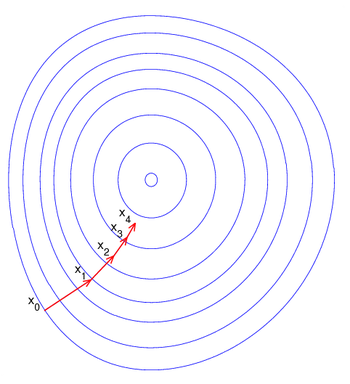
\includegraphics[scale=0.5]{./figures/figure_1.png}
\end{figure}

\section{示例}
\subsection{Rosenbrock}
首先我们给出函数:
\begin{equation}
	f(x,y)=(1-x)^2+100(y-x^2)^2
\end{equation}

该函数最小值在$(x,y)=(1,1)$处,$f(x,y)=0$。但该函数有一个狭小的弧形山谷,其中包含最小值。山谷的底部十分平坦,因此优化的过程十分缓慢。

\begin{figure}[H]
\centering
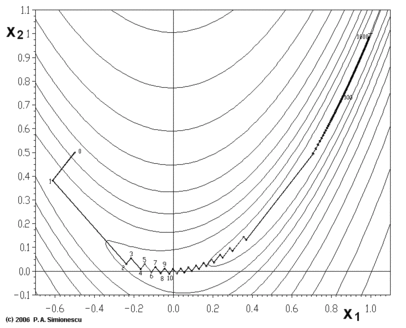
\includegraphics[scale=0.5]{./figures/figure_2.png}
\end{figure}


\subsection{案例总结}
梯度下降法的缺点包括:

1.靠近极小值时速度减慢,收敛速度比许多其他方法速度较慢;

2.直线搜索时会产生一些问题;

3.可能会呈“之字型”下降。

\section{应用}
\subsection{线性方程}
梯度下降可用于求解线性方程组,其被重新表示为二次最小化问题,例如,使用线性最小二乘法。
\begin{equation}
	A\mathbf x-\mathbf b=0
\end{equation}

在线性最小二乘意义上,定义为最小化函数
\begin{equation}
	F(\mathbf x)=\|A\mathbf x-\mathbf b\|^2
\end{equation}

在传统的线性最小二乘法中,使用欧几里德范数,在这种情况下
\begin{equation}
	\nabla F(\mathbf x)=2A^T(A\mathbf x-\mathbf b)
\end{equation}

在这种情况下,可以分析地执行线搜索最小化,在每次迭代中找到局部最优步长,并且已知局部最优的显式公式。

对于求解线性方程,该算法很少使用,共轭梯度法是最流行的替代方法之一。梯度下降的收敛速度取决于$A^TA$的最大特征值与最小特征值之比,而共轭梯度的收敛速度对于特征值,可以从预处理中受益。
\begin{figure}[H]
	\centering
	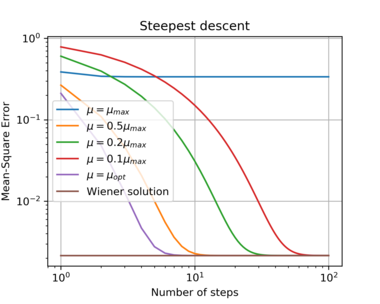
\includegraphics[scale=3]{./figures/figure-3.png}
\end{figure}
\subsection{非线性方程组}
对于
\begin{equation}
\begin{cases}
	3x_1-cos(x_2x_3)-\frac{3}{2}=0\\
	4x_1^2-625x_2^2+2x_2-1=0\\
	exp(-x_1x_2)+20x_3+\cfrac{10\pi-3}{3}=0
\end{cases}
\end{equation}

令
\begin{equation}
	G(\mathbf x)=\left[
\begin{array}{c}
          3 x_{1}-cos \left(x_{2} x_{3}\right)-\frac{3}{2}\\
          4 x_{1}^{2}-625 x_{2}^{2}+2 x_{2}-1 \\
         exp(-x_{1} x_{2})+20 x_{3}+\frac{10 \pi-3}{3}
\end{array}\right]
\end{equation}

此时,我们定义目标函数
\begin{equation}
	\begin{aligned}
	F(\mathbf x)&=\frac{1}{2} G^{T}(\mathbf x)G(\mathbf x)\\
		&=\frac{1}{2} [(3x_1-cos(x_2x_3)-\frac{3}{2})^2+4x_1^2-625x_2^2+2x_2-1)^2+(exp(-x_1x_2)+20x_3+\cfrac{10\pi-3}{3})^2]
	\end{aligned}
\end{equation}

令
$$\mathbf{x}^{(0)}=\mathbf{0}=\left[\begin{array}{l}{0} \\ {0} \\ {0}\end{array}\right]$$
得到
\begin{equation}
	\mathbf x^{(1)}=\mathbf 0-\gamma_0 \nabla F(\mathbf 0)=\mathbf 0-\gamma_{0} J_G(\mathbf 0)^{T} G(\mathbf 0)
\end{equation}

由此我们得到雅可比行列式$J_G$:
\begin{equation}
	J_G(\mathbf x)=
	\left[\begin{array}{ccc} 3 & sin(x_2 x_3) x_{3} & sin(x_2 x_3) x_2 \\ 
		8 x_1 & -1250 x_2+2 & 0 \\ 
		-x_2exp(-x_1 x_2) & -x_1 exp (-x_1 x_2)& 20
\end{array}\right]
\end{equation}
计算
$$J_{G}(\mathbf{0})=\left[\begin{array}{ccc}{3} & {0} & {0} \\ {0} & {2} & {0} \\ {0} & {0} & {20}\end{array}\right], \qquad G(\mathbf{0})=\left[\begin{array}{c}{-2.5} \\ {-1} \\ {10.472}\end{array}\right]$$
因此
$$\mathbf{x}^{(1)}=\mathbf{0}-\gamma_{0}\left[\begin{array}{c}{-7.5} \\ {-2} \\ {209.44}\end{array}\right]$$
及
$$F(\mathbf 0)=0.5\left((-2.5)^{2}+(-1)^{2}+(10.472)^{2}\right)=58.456$$

现在必须找到合适的$\gamma_0$,使得
$$F\left(\mathbf{x}^{(1)}\right) \leq F\left(\mathbf{x}^{(0)}\right)=F(\mathbf{0})$$
这可以通过各种线性搜索算法来完成。也可以简单的猜测$\gamma_0=0.001$给出了
$$\mathbf{x}^{(1)}=\left[\begin{array}{c}{0.0075} \\ {0.002} \\ {-0.20944}\end{array}\right]$$
以此值评估目标函数,得出
$$F\left(\mathbf{x}^{(1)}\right)=0.5((-2.47)^2+(-1.00)^2+(6.28)^2)=23.306$$

从$F(\mathbf 0)=580456$减少到$\mathbf{x}^{(1)}=23.306$目标函数的大幅减少。每一次计算都会降低其函数值,直到找到近似的值。
\section{评价}
梯度下降在任何维度的空间中进行,即使在无限维的空间中也是如此。在无限维空间中,搜索空间通常是一个函数空间,并且计算要最小化的函数的Fréchet导数以确定下降方向。
如果给定函数的不同方向上的曲率非常不同,则梯度下降可以进行许多次迭代来计算具有所需精度的局部最小值。对于这样的函数,采用改变空间的几何形状以形成像同心圆一样的函数水平集的预处理方法使其来逐步收敛收敛。然而,构造和应用预处理可能在计算上是麻烦的。

梯度下降可以与线性搜索组合,在每次迭代时找到局部最优步长$\gamma$。执行行搜索可能非常耗时。相反,使用固定的较小$\gamma$会产生较差的收敛。

基于牛顿方法和使用共轭梯度技术反向Hessian的方法可以是更好的替代方法。通常,这种方法在较少的迭代中收敛,但每次迭代的成本更高。以BFGS方法为例,其包括在每个步骤上计算矩阵,通过该矩阵将梯度向量乘以进入“更好”的方向,结合更复杂的线搜索算法,以找到$\gamma$的“最佳”值。对于计算机内存问题占主导地位的极大问题,应使用L-BFGS等有限记忆方法代替BFGS或最陡下降.

梯度下降可视为应用欧拉方法将常微分方程$x'(t)=-\nabla f(x(t))$的解作为梯度流。
\section{计算实例}
以Python代码为例,应用梯度下降算法来查找具有导数$f'(x)=4x^3-9x^2$的函数$f(x)x^4-3x^3+2$的最小值.

求解$4x^3-9x^2=0$并在解决方案中评估二阶导数表明该函数的平台点为0,全局最小值为$x=\frac{9}{4}$。

$x$的初始值取6,步长0.01,期望精度0.00001,最大迭代次数设置为10000。

最终得到极小值点为2.2499646074278457。
\section{拓展}
通过在约束集上包括投影,可以扩展梯度下降以处理约束。只有在计算机上有效计算投影时,此方法才可行。在适当的假设下,该方法收敛。该方法是单调包含的前后向算法的一个特定情况(包括凸规划和变分不等式)。

\subsection{快速梯度方法}
梯度下降的另一个延伸是由于Yurii Nesterov从1983年开始,并且随后被推广。他提供了一种简单的算法修改方法,可以更快地收敛凸问题。对于无约束平滑问题,该方法称为快速梯度法(FGM)或加速梯度法(AGM)。具体来说,如果可微函数$F$是凸的,并且$\nabla F$ 是Lipschitz,并且不假设$F$是强凸的,那么通过梯度下降法在每个步骤$k$生成的目标值的误差将受到$\mathcal O\left({\frac {1}{k}}\right)$的限制。使用Nesterov加速技术,误差在$\mathcal O\left({\tfrac {1}{k^{2}}}\right)$处降低.已知对于一阶优化方法,成本函数减小的速率$\mathcal O\left({k^{-2}}\right)$是最优的。 $\mathcal O \left({k^{-2}}\right)$降低成本函数对于一阶优化方法是最优的。然而,有机会通过减少常数因子来改进算法。优化梯度法(OGM)将该常数减少了两倍,是大规模问题的最优一阶方法。

对于约束或非平滑问题,Nesterov的FGM称为快速近端梯度法(FPGM),即近端梯度法的加速度。
\subsection{动量法}
另一个扩展,即降低陷入局部最小值的风险,以及在此过程可能会严重曲折的情况下大大加速收敛,是动量方法,它使用动量项类比“ 牛顿粒子在保守力场中穿过粘性介质的质量“。 该方法通常用作用于训练人工神经网络的反向传播算法的扩展。
\section{类比}
梯度下降背后的基本直觉可以通过假设情景来说明。一个人被困在山中,并试图下来(即试图找到最小值)。有大雾使能见度极低。因此,下山的路径是不可见的,所以他必须使用当地信息来找到最小值。他可以使用梯度下降的方法,该方法包括观察当前位置的山丘的陡度,然后沿着最陡下降的方向(即下坡)前进。如果他试图找到山顶(即最大值),那么他将沿着最陡上升(即上坡)的方向前进。使用这种方法,他最终会找到下山的路。然而,假设通过简单的观察,山的陡峭程度并不是立即显而易见的,而是需要一种精密的仪器来测量,此时人们碰巧拥有这种仪器。使用仪器测量山坡的陡度需要相当长的时间,因此如果他想在日落前下山,他应该尽量减少对仪器的使用。那么困难在于选择他应该测量山坡陡度的频率,以免偏离轨道。

在这个类比中,人代表算法,沿山的路径代表算法将探索的参数设置序列。山的陡度表示该点处的误差表面的斜率。用于测量陡度的仪器是微分(误差曲面的斜率可以通过取该点处的平方误差函数的导数来计算)。他选择行进的方向与该点处的误差表面的梯度一致。他在进行另一次测量之前旅行的时间量是算法的学习率。








\end{document}
